
% !TEX root =main.tex

\begin{center}
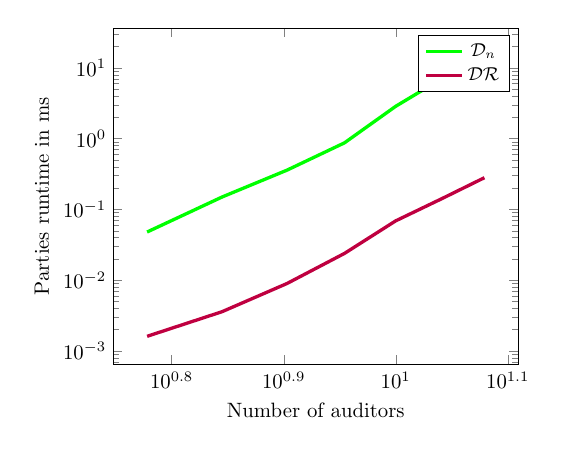
\begin{tikzpicture}[scale=.75]

\begin{loglogaxis}[
	xlabel={ Number of auditors },
	ylabel={ Parties runtime  in ms}
]


%\addplot[green,ultra thick] coordinates {
%  
%%     (1, 0.014)
%     (6, 0.033)
%     (7, 0.033)
%      (8, 0.033)
%      (9, 0.033)
%      (10, 0.033)
%      (11, 0.033)
%      (12, 0.033)
%
%};

\addplot[green, ultra thick] coordinates{

%        (1, 0.019)
       (6, 0.048)
       (7, 0.150)
      (8, 0.36)
      (9, 0.873)
      (10, 2.87)
      (11, 7.1)
      (12, 14.7)
};

\addplot[purple, ultra thick]  coordinates{

%  (1, 0.001)
        (6, 0.001611)
        (7, 0.00359)
      (8, 0.009)
      (9, 0.02389)
      (10, 0.069)
      (11, 0.1426)
      (12, 0.281)
};


\legend{\small $\mathcal{D}_{\st n}$,\small $\mathcal{DR}$}
\end{loglogaxis}
\end{tikzpicture}
\end{center}